\documentclass[main.tex]{subfiles}

\begin{document}
\section{Ze zničených SARS-CoV-2 vznikají nebezpečné “zombie” částice}
Fanoušci Soumraku mrtvých, Walking Dead nebo 28 časových úseků poté moc dobře ví, že sundat nemrtvou zombie není jen tak. Banda třiceti imunologů, mikrobiologů, fyziků, lékařů a~analytiků na to asi právě přišli taky. V trochu menším, ale neméně creepy měřítku.\par
Zatímco chodící mrtvole se dá utéct, schovat se do tanku nebo po ní fláknout vinylové LP, s~virem SARS-CoV-2 je to těžší. Kromě akutní fáze nemoci, která nás už stála miliony (a dále přičítáme) životů, je nádherným bonusem pro část přeživších syndrom dlouhého COVIDu. 
\subsection*{\enquote{Čeho že?}}
Objevuje se u~5-10\% nakažených virem. Projevuje se více než 200 symptomy. Mezi ně patří nevolnost, úzkosti, kognitivní problémy, dále problémy s~dechem, kardiovaskulárním systémem, imunitou a~svaly. Mezi další příznaky patří také chronické bolesti a~únava, která můžou zcela zabraňovat běžnému dennímu fungování. Dopodrobna jsme o~long covidu psali tady v~tomhle velmi autorizovaném textu.
\subsection*{\enquote{Tak už víme, čím to je?}}
Možná jsme na stopě. Jednou z~hlavních záhad je fakt, že symptomy přetrvávají i~po tom, co se tělo zbaví viru SARS-CoV-2. Yue Zhang a~její kolegové odhalili zombie verze viru u~SARS-Cov-2. Ne v~tom smyslu, že by virus způsoboval popkulturně známé žití a~hnití lidí, ale ve smyslu fragmentů virového obalu, které nám působí další brykule.\par
Jedním z~vážných projevů dlouhého COVIDu je zhoršená funkce imunitního systému, což může způsobovat spoustu dalších problémů. A zdá se, že v~tom mají prsty trosky rozflákaných virů.\par
Když se necítíte v~pohodě, zůstaňte doma, dejte si vychlazenou pintu a~počkejte, než se to všechno přežene. 
\subsection*{\enquote{Jak nás může ohrožovat mrtvý virus?}}
Jen tak na začátek – virus jako takový je považován za hranici mezi živým a~neživým. Nesplňuje totiž důležitou podmínku života – není schopen se sám rozmnožit. Jde jen o~nukleovou kyselinu zabalenou v~kapsidě. Prof. Jan Černý ho nazývá “balíček se špatnou zprávou”.\par
Tuhle zprávu virus dostane do buňky, hackne ji a~používá její mašinerii pro kopírování genů. Místo buněčné DNA, RNA či proteinů se tak kopírují nové viry. Tohle virus sám nezvládne, a~spousta vědátorů tedy viry za živé nepovažuje. \par
Ale i~vědátoři, kteří by virus živým nazvali se shodnou, že SARS-CoV-2 rozflákaný na malé kousky živý není už určitě. A právě ty kousky, na které virus rozšmelcovala naše imunita dost možná způsobují (alespoň část) symptomů dlouhého covidu. Hodně divné je, že některé imunitní buňky jsou zasaženy více než jiné. Důležité je, že takové kousky vznikají specificky po kontaktu s~naší imunitou, která virus rozsekává na specificky dlouhé fragmenty.
\subsection*{\enquote{Zombie kousky nám gryžou buňky?}}
Na naší imunitě se podílí spousta různých druhů buněk. Některé, třeba monocyty, jsou kulaté a~hladké. Oproti tomu dendritické buňky nebo T-lymfocyty mají velmi členitý povrch. Vědátoři na záhadu zaútočili matematickou simulací. Po férovce s~naší imunitou začaly kousky viru vlastnostmi připomínat AMP – antimikrobiální peptid. Molekulu, která je schopná dělat díry do bakterií, ale klidně i~do našich buněk. Užitečný nástroj, který používá většina živých tvorů. A zde i~jeden neživý.\par
Vlastnostmi penetrovat buňky to nekončí. Fragmenty, nazvané xeno-AMPs mají dokonalý tvar na to, aby zapadly do prohlubní na těch imunitních buňkách, které jsou členité. \par
Takže po hladkých buňkách xeno-AMP částice sklouznou, zatímco do vrásčitých ze zahryzávají a~dělají do nich díry.
\subsection*{\enquote{A co na to ty naše buňky?}}
\begin{wrapfigure}{r}{0.4\linewidth}
  \centering
  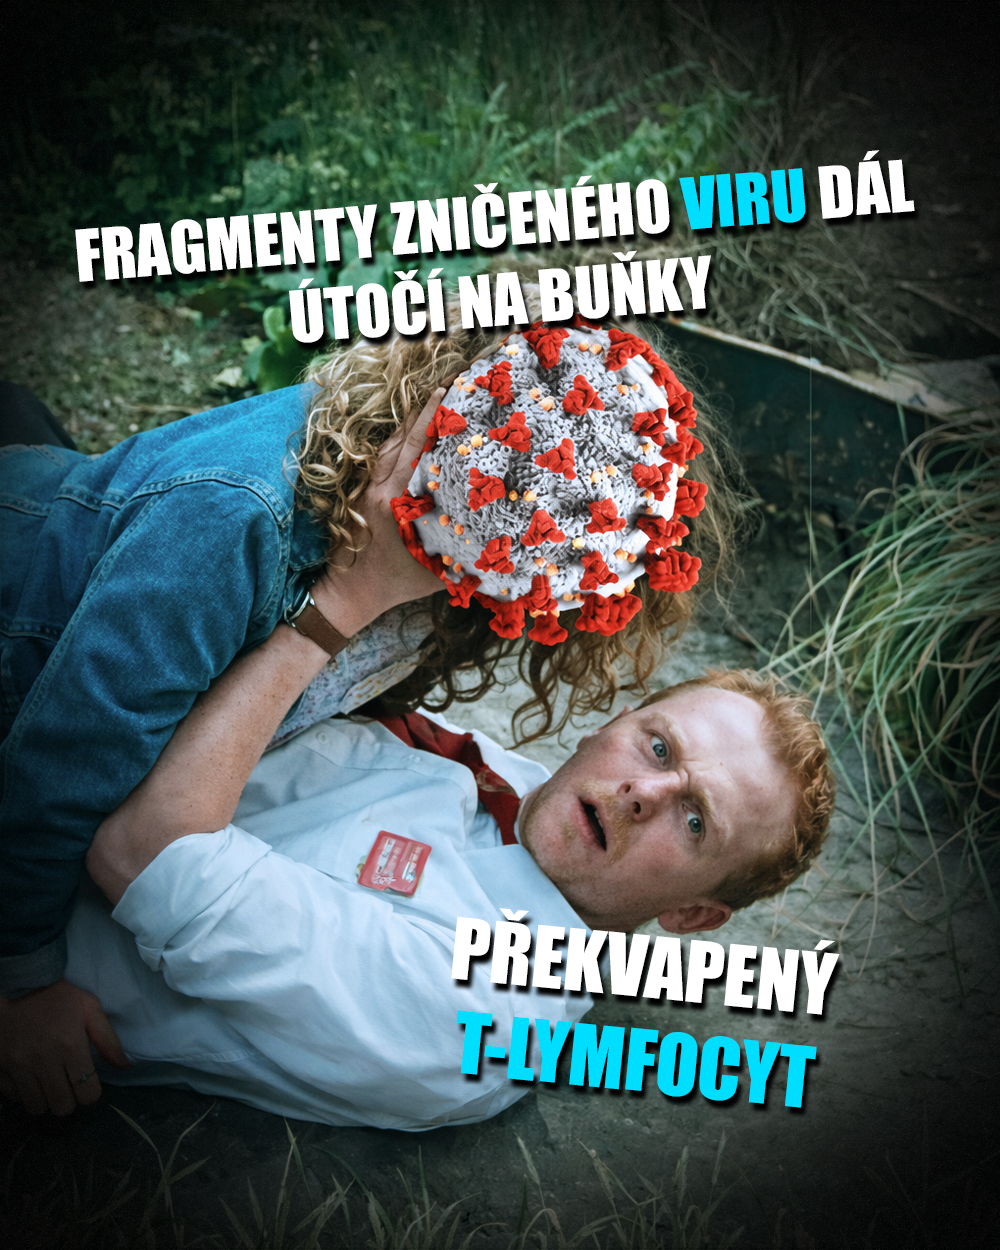
\includegraphics[width=0.95\linewidth]{sars.png}
\end{wrapfigure}
Jeden tým modeloval, druhý testoval. Vědátoři a~vědátorky na čerstvé imunitní buňky z~krve zdravých dárců pod frcli virové trosky. T-lymfocyty po dodávce zombie částic umíraly 6x častěji, dendritické buňky 3x častěji, plazmacytoidní dendritické buňky dokonce 70x častěji. Hladké monocyty a~neutrofily vyšly bez újmy. \par
Jako bonus tyto výsledky louskají další záhadu – proč nakažlivější varianta Omikron nemívá až tak těžký průběh? Stavební kameny proteinů téhle varianty viru se drobně liší. Zmutováním jedné jediné aminokyseliny dojde ke změně polarity zombie kousku. A už klesá schopnost škodit, a~dopad není až tak velký (byť to furt není žádná lahoda).
\subsection*{\enquote{K čemu nám to je?}}
Přicházíme na kloub záhadě zvané dlouhý COVID. Máme k~dispozici další parametr, se kterým můžeme počítat v~diagnostice a~léčbě COVID-19 a~možná i~dalších onemocnění, způsobených podobným mechanismem.\par
A taky to ještě více pozvedává význam očkování – to, že očkovaní nemají tyhle problémy, víme ze statistik. Pokud už se nakazíme, je lepší mít připravenou armádu imunitních buněk vycvičených vakcínou. Tak se můžeme viru zbavit rychle a~vyrobit z~nepřátelské armády co nejnižší počet xeno-AMPs.\par
Alternativní (a dost debilní) nápad promoření může vést k~masivnějšímu zamoření našich orgánů zombie částicemi. Což vám, i~když přežijete, rozhodí papuč, imunitu, a~sekundárně může vést k~plejádě dalších symptomů dlouhého COVIDu.
\newpage
\end{document}